%! Author = maxx
%! Date = 11/27/24

% Preamble
\documentclass[12pt]{report}

\usepackage[a4paper, left=2.5cm, right=2.5cm, top=3cm, bottom=3cm]{geometry}
\usepackage{graphicx}
\usepackage{pdfpages}
\usepackage{glossaries}
\usepackage{titling}
\setlength{\parindent}{0pt}


\title{POO - Laboratoire 7 \\ \large Calculatrice}
\author{Lestiboudois Maxime \& Parisod Nathan}
\date{27/11/2024}

% Redéfinir \maketitle pour inclure l'image sous le titre
\pretitle{\begin{center}\Huge\bfseries}
\posttitle{\par\end{center}\vspace{0.5cm}
\begin{center}

\includegraphics[scale = 0.2]{images/SingeCalculatrice}
\end{center}\vspace{0.5cm}}

% Document
\begin{document}
    \maketitle
    \tableofcontents
    \newpage

%%%%%%%%%%%%%%%%%%%%
%%  Introduction  %%
%%%%%%%%%%%%%%%%%%%%

    \section*{Introduction}
    \addcontentsline{toc}{section}{Introduction}
    Dans ce laboratoire, nous avons implémenté la logique d'une calculatrice utilisant la notation polonaise inversée.
    L'interface nous étant déjà fournie, nous nous sommes concentrés sur l'aspect fonctionnel de la calculatrice.
    \newline Nous avons également implémenter une extension de notre calculatrice afin de pouvoir l'utiliser directement
    dans un terminal.

%%%%%%%%%%%%%%%%%%%%
%Cahier des charges%
%%%%%%%%%%%%%%%%%%%%
    \section*{Cahier des charges}
    \addcontentsline{toc}{section}{Cahier des charges}
        \subsection*{Objectif du Projet}
        \addcontentsline{toc}{subsection}{Objectif du Projet}
        Créer une calculatrice fonctionnant en notation polonaise inverse (Reverse Polish Notation - RPN). Elle doit inclure une interface graphique (GUI) et un mode console, réutilisant les mêmes classes et principes. Le projet doit suivre une architecture Modèle-Vue-Contrôleur (MVC).

        \subsection*{Spécifications Fonctionnelles}
        \addcontentsline{toc}{subsection}{Spécifications Fonctionnelles}
            \subsubsection*{Interface Graphique (GUI)}
            \addcontentsline{toc}{subsubsection}{Interface Graphique (GUI)}
                \begin{itemize}
                    \item Implémenter une interface utilisateur dans la classe JCalculator.
                    \item Boutons requis :
                    \begin{itemize}
                        \item Chiffres : 0-9.
                        \item Opérations unaires : sqrt, 1/x, \verb|x^2|.
                        \item Opérations binaires : +, -, *, /.
                        \item Autres boutons :
                        \begin{itemize}
                            \item MR : récupérer une valeur en mémoire.
                            \item MS : stocker une valeur en mémoire.
                            \item \verb|<=| : backspace pour supprimer le dernier caractère.
                            \item CE : réinitialiser l’affichage.
                            \item C : réinitialiser l’affichage et vider la pile.
                            \item Ent : placer la valeur courante sur la pile.
                            \item +/- : changer le signe de la valeur courante.
                            \item . : pour les nombres décimaux.
                        \end{itemize}
                    \end{itemize}

                    \item Affichage :
                    \begin{itemize}
                        \item Zone de texte (JTextField) pour la valeur courante.
                        \item Liste (JList) pour visualiser la pile.
                    \end{itemize}

                    \item Mise à jour de l'affichage après chaque opération via une méthode update().
                \end{itemize}
            \subsubsection*{Mode Console}
            \addcontentsline{toc}{subsubsection}{Mode Console}
                \begin{itemize}
                    \item Développer une classe Calculator permettant une interaction textuelle.
                    \item Commandes utilisateur :
                    \begin{itemize}
                        \item Saisir un nombre pour l’ajouter à la pile.
                        \item Entrer une opération (+, sqrt, etc.).
                        \item exit : quitter la calculatrice.
                    \end{itemize}

                    \item Fonctionnalités similaires à la version graphique :
                    \begin{itemize}
                        \item Gestion de la pile.
                        \item Support des opérations unaires, binaires et de mémoire.
                    \end{itemize}
                \end{itemize}

            \subsubsection*{Gestion des Données et Opérations}
            \addcontentsline{toc}{subsubsection}{Gestion des Données et Opérations}
                \begin{itemize}
                    \item Pile personnalisée (Stack) :
                    \begin{itemize}
                        \item Empiler une valeur.
                        \item Désempiler une valeur.
                        \item Obtenir l’état actuel de la pile sous forme de tableau.
                        \item Fournir un itérateur pour parcourir la pile.
                        \item Implémentée avec une liste chaînée sans structures Java préconstruites.
                    \end{itemize}

                    \item État interne (State) :
                    \begin{itemize}
                        \item Stocker :
                        \begin{itemize}
                            \item Valeur courante.
                            \item Pile des valeurs.
                            \item État d’erreur.
                        \end{itemize}

                        \item Fournir des méthodes pour gérer et manipuler ces données.
                    \end{itemize}
                \end{itemize}

            \subsection*{Spécifications Techniques}
            \addcontentsline{toc}{subsection}{Spécifications Techniques}
                \subsubsection*{Architecture MVC}
                \addcontentsline{toc}{subsubsection}{Architexture MVC}
                    \begin{itemize}
                        \item Modèle (State) :
                        \begin{itemize}
                            \item Indépendant de l’interface graphique.
                            \item Stocke les données et implémente la logique de calcul.
                        \end{itemize}

                        \item Vue (JCalculator) :
                        \begin{itemize}
                            \item Interface utilisateur graphique basée sur Swing.
                            \item Réagit aux changements dans le modèle.
                        \end{itemize}

                        \item Contrôleurs (Operator) :
                        \begin{itemize}
                            \item Boutons dans l’interface graphique agissant comme des contrôleurs.
                            \item Appel de la méthode execute() d’un objet Operator.
                        \end{itemize}
                    \end{itemize}
                \subsubsection*{Hiérarchie des Classes}
                \addcontentsline{toc}{subsubsection}{Hiérarchie des Classes}
                    \begin{itemize}
                        \item Classe générique Stack pour représenter une pile.
                        \item Classe State pour l'état interne.
                        \item Hiérarchie Operator :
                        \begin{itemize}
                            \item Classe de base Operator :
                            \begin{itemize}
                                \item Méthode execute().
                            \end{itemize}

                            \item Sous-classes spécialisées :
                            \begin{itemize}
                                \item NumberOperator, AdditionOperator, SqrtOperator, etc.
                            \end{itemize}
                        \end{itemize}

                        \item Classe JCalculator pour l'interface graphique.
                        \item Classe Calculator pour le mode console.
                    \end{itemize}
            \subsection*{Contraintes}
            \addcontentsline{toc}{subsection}{Contraintes}
                \begin{itemize}
                    \item Aucune utilisation de switch ou de if pour sélectionner l'opération dans Operator.
                    \item Pas de propriétés statiques pour le stockage des données.
                    \item Le code doit être modulaire et réutilisable.
                    \item Respect des principes de conception objet.
                \end{itemize}
            \subsection*{Tests}
            \addcontentsline{toc}{subsection}{Tests}
                \begin{itemize}
                    \item Élaborer une grille de tests couvrant :
                    \begin{itemize}
                        \item Les opérations unaires et binaires.
                        \item Les erreurs (ex. : division par zéro, pile vide).
                        \item Le stockage et rappel de mémoire.
                        \item La compatibilité entre le mode console et GUI.
                    \end{itemize}

                    \item Inclure des cas limites et des tests d'intégration.
                \end{itemize}

%%%%%%%%%%%%%%%%%%%%
%%  Schéma UML  %%
%%%%%%%%%%%%%%%%%%%%
    \section*{Schéma UML}
    \addcontentsline{toc}{section}{Schéma UML}
    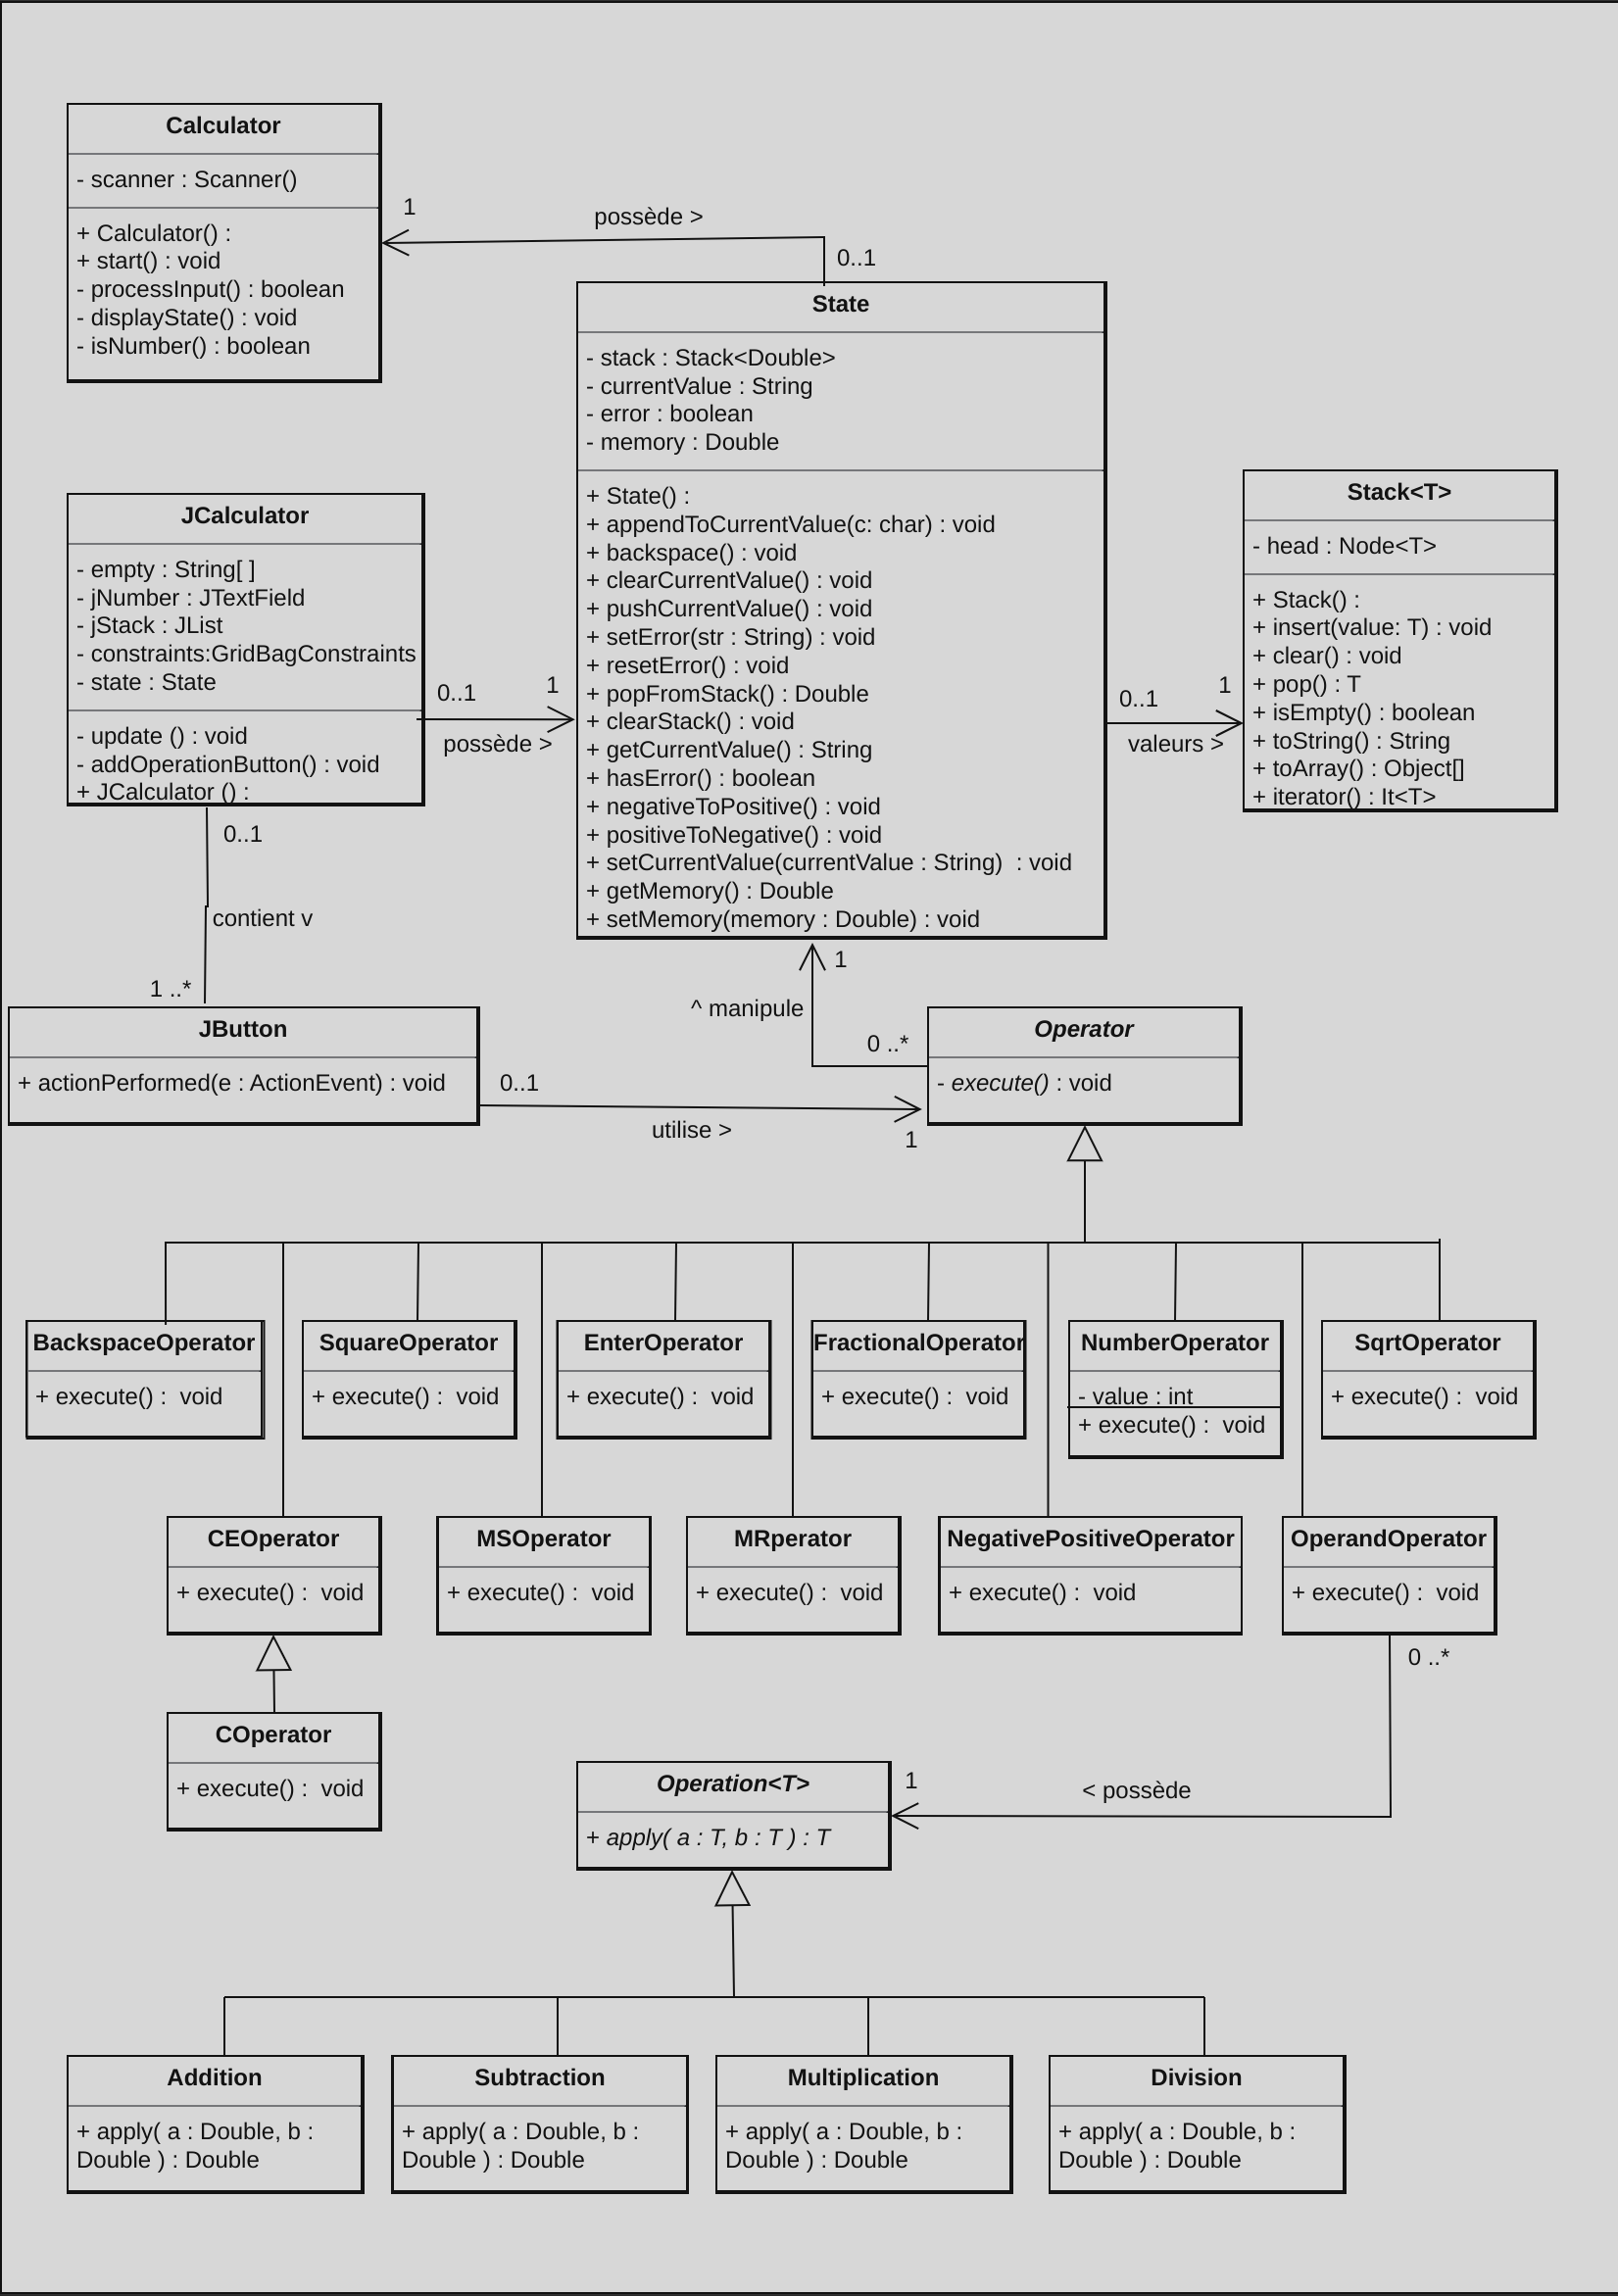
\includegraphics[scale=0.3]{images/diagram}

%%%%%%%%%%%%%%%%%%%%
%%  Listing code  %%
%%%%%%%%%%%%%%%%%%%%
    \section*{Listing du code}
    \addcontentsline{toc}{section}{Listing du code}
    %\includepdf[page=-, pagecommand={\thispagestyle{plain}}]{src.pdf}

%%%%%%%%%%%%%%%%%%%%
% Choix Conception %
%%%%%%%%%%%%%%%%%%%%
    \section*{Choix de conception}
    \addcontentsline{toc}{section}{Choix de conception}
        \subsection*{Les opérateurs}
        \addcontentsline{toc}{subsection}{Les opérateurs}
            Nous avons reçu un dossier "starter" fourni par le corps professoral. Dans ce dossier, nous avons trouvé le
    fichier Operator, contenant la classe abstraite Operator, qui nous a servit de base pour construire tous les opérateurs (fonctionnalités des boutons) de notre
    calculatrice.
    \newline Nos opérateurs sont tous, sans exception, des classes enfants de la classe abstraite Operator, elles redéfinissent
    donc toutes la méthode abstraite execute() de la super-classe.
    Nous avons choisi que chaque opérateur, excepté les opérateurs d'opérations arithmétiques, serait un enfant direct de la
    super-classe Operator.
    \newline
    Par ailleurs, chaque classe-enfant ne comporte aucun attribut, excepté les classe NumberOperator et OperantOperator.
    NumberOperator possède un attribut privé et final. Ce choix nous permet de ne pas redéfinir une nouvelle classe pour chaque
    chiffre, ces derniers étant définis lors de l'instanciation de l'objet via le constructeur.
    \newline Nous discuterons de la classe Operand Operator dans le point suivant.

        \subsection*{Opérations arithmétiques}
        \addcontentsline{toc}{subsection}{Opérations arithmétiques}
            Les opérations arithmétiques entre les différentes valeurs de la stack se font via la classe OperandOperaor.
    \newline Cette classe prend comme attribut une instance de la classe Operation\verb|<T>| (ici T est un objet de type Double).
    La classe Operation<T> est une classe publique abstraite qui implémente la méthode (abstraite également) apply(T a, T b).
    L'appel à cette fonction depuis OperandOperator permet de traiter les opérations arithmétiques proposées par les classes
    enfants de Operation.
    \newline Parmi les classes enfants de Operation, nous avons choisi de n'implémenter que les classes suivantes:
    \begin{itemize}
        \item Addition
        \item Subtraction
        \item Multiplication
        \item Division
    \end{itemize}
    Nous n'avons pas besoin de plus pour notre calculatrice, cependant nous gardons ainsi la possibilité d'implémenter d'autres
    opérations utilisant deux opérandes de manière simple et optimisée.

        \subsection*{Gestion d'écriture et de mémoire}
        \addcontentsline{toc}{subsection}{Gestion d'écriture et de mémoire}
            Comme demandé dans le cahier des charges, notre calculatrice comprend un bouton "C", permettant d'effacer ce qui était
    en train d'être écrit (classe CEOperator), ainsi qu'un bouton reprenant cette même fonctionnalité et supprimant par la même occasion le
    contenu de la stack (pile) de la calculatrice (classe COperator). Afin d'éviter toute redondance de code, nous avons décidé que
    la classe COperator serait une sous-classe de la classe CEOperator. Ainsi, un simple appel à la super méthode nous permet
    d'accéder aux fonctionnalités de la super-classe CEOperator.
    \newline Notre calculatrice implémente également une fonctionnalité mémoire avec les boutons MR et MS. MS permet de
    sauver dans l'attribut memory de la classe State, un objet de type Double. Le bouton MR permet de récupérer la valeur
    sauvée dans la mémoire. Ces deux fonctionnalités fonctionnement respectivement grâce aux classes MSOperator et MROperator.
    \newline Nous avons choisi que lorsque la mémoire serait récupérée, la valeur contenue en mémoire ne serait pas affecter et resterait
    la même. De même lorsque les boutons C ou CE seraient sélectionnés, la mémoire n'est pas affectée par l'exécution des autres
    fonctionnalités.

    \subsection*{Stack}
    \addcontentsline{toc}{subsection}{Stack}
        la classe Stack\verb|<T>| est indispensable au bon fonctionnnement de la calculatrice. C'est en effet l'élément qui
    sert à stocker toutes les valeurs entrées par l'utilisateur et l'endroit d'où les valeurs sont tirées pour être par la suite traitées (calculées).
    \newline Ayant nous-même créé la stack, nous avons décidé de créer une classe Node, représentant les éléments présents dans la Stack.
    La Stack en elle-même représente alors une chaîne, permettant de contrôler l'ordre d'arrivée et de sortie des éléments.

    \subsection*{State et Operator}
    \addcontentsline{toc}{subsection}{State et Operator}
        la classe State est celle qui centralise toutes les informations liées à la calculatrice. Elle prend comme seul attribut
    une instance de la classe Stack. La classe State renvoie les données qui seront affichées par la calculatrice, données qui
    sont modifiées par les instances des objets de type Operator.





%%%%%%%%%%%%%%%%%%%%
% Tests effectués %
%%%%%%%%%%%%%%%%%%%%
    \section*{Tests effectués}
    \addcontentsline{toc}{section}{Tests effectués}

%%%%%%%%%%%%%%%%%%%%
%    Conclusion    %
%%%%%%%%%%%%%%%%%%%%
    \section*{Conclusion}
    \addcontentsline{toc}{section}{Conclusion}
        Nos deux programmes/calculatrices marchent tel que nous le souhaitons. Nous avons grâce à ce laboratoire pu apprendre
    comment fonctionne une architecture MVC et avons pu mettre en pratique notre code dans deux contextes différents, une fois sur
    l'interface graphique et la seconde fois dans l'extension, en mode console. \newline Nous avons ainsi que tout code bien construit
    peut être réutiliser dans plusieurs contextes différents.

\end{document}

